\documentclass[a4j,twocolumn,dvipdfmx,autodetect-engine]{jsarticle}

\usepackage[top=30truemm]{geometry}
\usepackage{here}
\usepackage[dvipdfmx]{graphicx}

\begin{document}

\title{時間と共に変化する多重集合に対するmin-hashの高速計算}
\author{古賀研究室  1610615  三原寛寿}
\maketitle

\section{集合間類似検索}
近年,集合間類似検索に注目がある.そして,この集合間類似検索とはクエリ集合と類似している集合をデータベースから検索する問題である.

集合間類似検索は集合間類似度を何度も計算する必要があり,Jaccard係数(1)を用いる.
\begin{center}
$sim(S,Q)=$ $ \frac {|S| \cap {|Q|} } {|S| \cup {|Q|} }$
\end{center}

Jaccard係数とは,2つの集合に含まれ散る要素のうち共通要素が占める割合である.しかし,Jaccard係数による類似度の厳密計算は2つの集合間の類似度を計算するオーバーヘッドが大きい.そのため,Jaccard係数を高速に近似計算する方法がある.それは集合AとBのコンパクトなスケッチを生成し,スケッチ間でJaccard係数を近似計算することである.スケッチの生成にはMin-hash[2]が使用される.


\section{Min-Hash}
Min-hashとは集合に対する確率的なハッシュ関数である.Min-hashの計算方法を説明する.アルファベット集合$λ=\{x_1,x_2,…,x_|λ|\}$とする.λのアルファベットに対して,ランダムな値$π(e)$を割り当てる.

\begin{figure}[H]
  \centering
  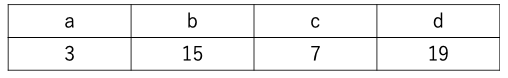
\includegraphics[width=6cm]{1wariate.png}
  \caption{集合の割り当て表}
\end{figure}

集合Aのハッシュ値はAに含まれる要素の中で割り当て値が最小値のもを使用する.
\begin{center}
$h(A)=\min_{e \in \mbox{A}} π(e)$
\end{center}

\subsection{多重集合に対するMin-hash}
多重集合とは,集合を同一集合の要素を複数持てるようにしたものである.例えば,$\{a,b,b,c,c,d,d\}$という集合である.多重集合の場合,同じアルファベットを複数含む場合には異なる割り当て値を与える.
\begin{figure}[H]
  \centering
  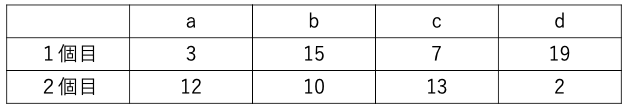
\includegraphics[width=6cm]{2wariate.png}
  \caption{多重集合の割り当て表}
\end{figure}

多重集合でのMin-hashの計算も集合の時と同じように最小値を選ぶ.

\section{動的に変化する集合に対する類似度計算}
最近では動的に変化する集合に対する類似検索も注目されてる.動的集合に対する類似検索の1つの例として,ストリームデータの類似検索がある.ストリームデータとは毎時刻アルファベットが1つ到着するデータであり,直近のw個の要素をスライディングウインドウとして,動的に変化する集合とみなせる.


\subsection{時間と共に変化する集合に対するハッシュ値更新}
Datarら[1]は時間と共に変化する集合に対するハッシュ値更新を効率よく行う方法を提案した.

Datarらのやり方は過去の計算結果を利用するやり方である.これは最小値になり得ない要素を消し,更新時に調べる要素数を削減するということだ.スライディングウインドウでは,自分より後ろに小さい値を持つ要素が存在する限り,その値は先に抜け,必ず最小値になる要素はない.
そして,最小値になりうる要素をMinlistに保持する.

Minlistは単調増加に保たれ,先頭の最小値がハッシュ値となる.

\begin{figure}[H]
  \centering
  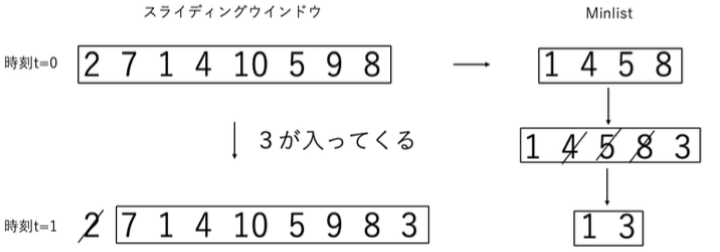
\includegraphics[width=5cm]{Minlist.png}
  \caption{最小値の候補リストMinlistの作成}
\end{figure}

\section{本研究の目的}
本研究の目的は,Datar[1]らによる動的に変化する集合に対してのハッシュ値更新のアルゴリズムを動的多重集合に拡張することである.

\section{多重集合になったことの難しさ}
多重集合では,スライディングウインドウ内の個数によって,割り当て値が変化する.

Minlist内で同一アルファベットを1つ保持すれば済むように,割り当て値表を修正する.1つのアルファベットに注目して,2個目の割り当て値が1大きい場合,1個目の割り当て値に書き換える.

\section{ウインドウ更新の処理}
多重集合にDatarらのやり方を適用する場合,ウインドウの更新の処理も難しくなる.
まず,要素をウインドウに追加する処理では,入ってきた要素の割り当て値と比べてMinlistを更新するのではなく,入ってきた要素と同じアルファベットを持つ要素のウインドウ内の一番古い要素の割り当て値と比べて,Minlistを更新する.

\section{処理時間についての実験と評価}
クエリが変化せず,データベースを毎時刻更新する問題設定を用いた.アルファベットの多重度の上限値$L=\{2,3,4,5\}$と変化させた.データベース内の集合数は1000とした.時刻$t=1$から1000まで進め,1000回の類似度top-10検索にかかる合計の処理時間を比較した.
\begin{figure}[H]
  \centering
  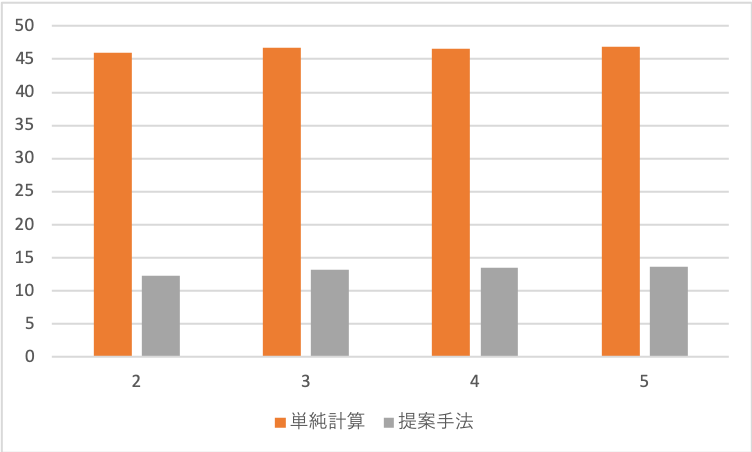
\includegraphics[width=6cm]{hikaku.png}
  \caption{割り当て表の更新}
\end{figure}

結果として,単純手法より提案手法の方が処理時間が早いことがわかった.

\section{まとめ}
本論文では,動的に変化する集合に対して,Min-hash値を更新するアルゴリズムを多重集合へ対応するように拡張した.単純手法より,多重集合に対して,高速に類似度を近似計算できることを示せた.

今後の課題としては,データを保持するためにヒストグラムを多用して,メモリを多く使用しているので,ヒストグラムを使用せずに類似度計算を行い,メモリを削減させることである.

\section{参考文献}
[1]Mayur Datar and S Muthukrishnan "Estimating Rarity and Similarity over Data Stream Window" AT\&T Research, Florham Park NJ, USA

[2]岡野原 大輔, “MinHash による高速な類似検索”, https://research.preferred. jp/2011/02/minhash/
\end{document}
